\documentclass[11pt]{article}
\usepackage[margin=1in]{geometry}
\usepackage{amsmath,amssymb}
\usepackage{booktabs}
\usepackage{graphicx}
\usepackage{natbib}
\usepackage[hidelinks]{hyperref}
\usepackage{xcolor}
\usepackage{caption}
\captionsetup{font=small}
\bibliographystyle{plainnat}
\newcommand{\kappaOne}{1.60}
\newcommand{\rsqOne}{-0.19}
\newcommand{\nOne}{22}
\newcommand{\maeOne}{0.18}
\newcommand{\rhoOne}{0.48}
\newcommand{\plugN}{21}
\newcommand{\plugMAE}{0.049}
\newcommand{\plugRho}{0.95}
\newcommand{\plugAgree}{30}
\newcommand{\plugTot}{32}
\newcommand{\plugMAEfive}{0.038}
\newcommand{\plugMAEnn}{0.059}
\newcommand{\negNF}{22}
\newcommand{\nDense}{24}
\newcommand{\recMed}{62}
\newcommand{\recMin}{32}
\newcommand{\recMax}{730}
\newcommand{\naiveMin}{-2.68}
\newcommand{\naiveMax}{-0.11}
\newcommand{\ssMin}{15}
\newcommand{\ssMax}{72}
\newcommand{\ssBmMax}{8}
\newcommand{\rqPosThree}{20}
\newcommand{\qDiffMax}{0.10}
\newcommand{\crossMin}{0.11}
\newcommand{\crossMax}{0.86}
\newcommand{\totKB}{446,641}
\newcommand{\totAsks}{23,703}
\newcommand{\totRep}{10,558}
\newcommand{\rqTurned}{9}
\newcommand{\recMedStill}{52}
\newcommand{\nStill}{15}
\newcommand{\recMinStill}{32}
\newcommand{\recMaxStill}{76}

\newcommand{\dNNBgeAsk}{-1.89}
\newcommand{\dThBgeAsk}{-0.21}
\newcommand{\negBgeAsk}{12}
\newcommand{\selfBgeAsk}{56}
\newcommand{\capBgeAsk}{74}
\newcommand{\capwBgeAsk}{72}
\newcommand{\stealBgeAsk}{26}
\newcommand{\medBgeAsk}{0.15}
\newcommand{\dNNBgeDoc}{+0.00}
\newcommand{\dThBgeDoc}{+0.00}
\newcommand{\negBgeDoc}{0}
\newcommand{\selfBgeDoc}{0}
\newcommand{\capBgeDoc}{51}
\newcommand{\capwBgeDoc}{51}
\newcommand{\stealBgeDoc}{0}
\newcommand{\medBgeDoc}{$>$0.95}
\newcommand{\dNNBgeAskdoc}{-0.02}
\newcommand{\dThBgeAskdoc}{+0.14}
\newcommand{\negBgeAskdoc}{1}
\newcommand{\selfBgeAskdoc}{14}
\newcommand{\capBgeAskdoc}{52}
\newcommand{\capwBgeAskdoc}{49}
\newcommand{\stealBgeAskdoc}{3}
\newcommand{\medBgeAskdoc}{0.75}
\newcommand{\dNNMiniAsk}{-0.58}
\newcommand{\dThMiniAsk}{+0.29}
\newcommand{\negMiniAsk}{10}
\newcommand{\selfMiniAsk}{33}
\newcommand{\capMiniAsk}{58}
\newcommand{\capwMiniAsk}{55}
\newcommand{\stealMiniAsk}{12}
\newcommand{\medMiniAsk}{0.43}
\newcommand{\dNNMiniDoc}{+0.00}
\newcommand{\dThMiniDoc}{+0.00}
\newcommand{\negMiniDoc}{0}
\newcommand{\selfMiniDoc}{0}
\newcommand{\capMiniDoc}{47}
\newcommand{\capwMiniDoc}{47}
\newcommand{\stealMiniDoc}{0}
\newcommand{\medMiniDoc}{$>$0.95}
\newcommand{\dNNMiniAskdoc}{-0.02}
\newcommand{\dThMiniAskdoc}{+0.20}
\newcommand{\negMiniAskdoc}{4}
\newcommand{\selfMiniAskdoc}{18}
\newcommand{\capMiniAskdoc}{53}
\newcommand{\capwMiniAskdoc}{49}
\newcommand{\stealMiniAskdoc}{3}
\newcommand{\medMiniAskdoc}{0.80}
\newcommand{\dNNBmAsk}{-0.00}
\newcommand{\dThBmAsk}{+0.03}
\newcommand{\negBmAsk}{4}
\newcommand{\selfBmAsk}{4}
\newcommand{\capBmAsk}{30}
\newcommand{\capwBmAsk}{29}
\newcommand{\stealBmAsk}{1}
\newcommand{\medBmAsk}{$>$0.95}
\newcommand{\dNNBmDoc}{+0.00}
\newcommand{\dThBmDoc}{+0.00}
\newcommand{\negBmDoc}{0}
\newcommand{\selfBmDoc}{0}
\newcommand{\capBmDoc}{47}
\newcommand{\capwBmDoc}{47}
\newcommand{\stealBmDoc}{0}
\newcommand{\medBmDoc}{$>$0.95}
\newcommand{\dNNBmAskdoc}{+0.01}
\newcommand{\dThBmAskdoc}{+0.07}
\newcommand{\negBmAskdoc}{2}
\newcommand{\selfBmAskdoc}{13}
\newcommand{\capBmAskdoc}{52}
\newcommand{\capwBmAskdoc}{49}
\newcommand{\stealBmAskdoc}{2}
\newcommand{\medBmAskdoc}{$>$0.95}
\newcommand{\diffMedShift}{-0.06}
\newcommand{\diffUp}{0}
\newcommand{\diffDown}{7}
\newcommand{\diffMinShift}{-0.27}
\newcommand{\diffMaxShift}{+0.19}
\newcommand{\diffDnnConst}{-1.23}
\newcommand{\diffDnnDiff}{-1.27}
\newcommand{\diffNegNN}{21}
\newcommand{\realizedNN}{0.95}
\newcommand{\oosNAskTh}{39}
\newcommand{\oosMAEAskTh}{0.085}
\newcommand{\oosRhoAskTh}{0.88}
\newcommand{\oosSameAskTh}{54}
\newcommand{\oosDefAskTh}{64}
\newcommand{\oosNAskFi}{36}
\newcommand{\oosMAEAskFi}{0.102}
\newcommand{\oosRhoAskFi}{0.79}
\newcommand{\oosSameAskFi}{51}
\newcommand{\oosDefAskFi}{68}
\newcommand{\oosNAskdocTh}{23}
\newcommand{\oosMAEAskdocTh}{0.248}
\newcommand{\oosRhoAskdocTh}{0.00}
\newcommand{\oosSameAskdocTh}{42}
\newcommand{\oosDefAskdocTh}{57}
\newcommand{\blAskNaive}{-1.23}
\newcommand{\blThAskNaive}{+0.04}
\newcommand{\blNNAskNaive}{0}
\newcommand{\blKeptAskNaive}{100}
\newcommand{\blAskDem}{-0.36}
\newcommand{\blThAskDem}{+0.51}
\newcommand{\blNNAskDem}{9}
\newcommand{\blKeptAskDem}{100}
\newcommand{\blAskQuar}{-0.37}
\newcommand{\blThAskQuar}{+0.65}
\newcommand{\blNNAskQuar}{9}
\newcommand{\blKeptAskQuar}{100}
\newcommand{\blAskGate}{-0.83}
\newcommand{\blThAskGate}{+0.16}
\newcommand{\blNNAskGate}{2}
\newcommand{\blKeptAskGate}{63}
\newcommand{\blAskFoot}{-1.09}
\newcommand{\blThAskFoot}{-0.04}
\newcommand{\blNNAskFoot}{0}
\newcommand{\blKeptAskFoot}{79}
\newcommand{\blDocNaive}{+0.00}
\newcommand{\blThDocNaive}{+0.00}
\newcommand{\blNNDocNaive}{24}
\newcommand{\blKeptDocNaive}{100}
\newcommand{\blDocDem}{+0.00}
\newcommand{\blThDocDem}{+0.00}
\newcommand{\blNNDocDem}{24}
\newcommand{\blKeptDocDem}{100}
\newcommand{\blDocQuar}{-0.00}
\newcommand{\blThDocQuar}{+0.05}
\newcommand{\blNNDocQuar}{16}
\newcommand{\blKeptDocQuar}{100}
\newcommand{\blDocGate}{+0.00}
\newcommand{\blThDocGate}{+0.00}
\newcommand{\blNNDocGate}{24}
\newcommand{\blKeptDocGate}{55}
\newcommand{\blDocFoot}{+0.00}
\newcommand{\blThDocFoot}{+0.00}
\newcommand{\blNNDocFoot}{24}
\newcommand{\blKeptDocFoot}{85}
\newcommand{\blAskdocNaive}{-0.02}
\newcommand{\blThAskdocNaive}{+0.17}
\newcommand{\blNNAskdocNaive}{7}
\newcommand{\blKeptAskdocNaive}{100}
\newcommand{\blAskdocDem}{+0.12}
\newcommand{\blThAskdocDem}{+0.23}
\newcommand{\blNNAskdocDem}{20}
\newcommand{\blKeptAskdocDem}{100}
\newcommand{\blAskdocQuar}{+0.11}
\newcommand{\blThAskdocQuar}{+0.29}
\newcommand{\blNNAskdocQuar}{20}
\newcommand{\blKeptAskdocQuar}{100}
\newcommand{\blAskdocGate}{+0.02}
\newcommand{\blThAskdocGate}{+0.14}
\newcommand{\blNNAskdocGate}{14}
\newcommand{\blKeptAskdocGate}{56}
\newcommand{\blAskdocFoot}{-0.04}
\newcommand{\blThAskdocFoot}{+0.13}
\newcommand{\blNNAskdocFoot}{8}
\newcommand{\blKeptAskdocFoot}{90}
\newcommand{\ceGainMin}{-0.8}
\newcommand{\ceGainMax}{0.9}
\newcommand{\ceN}{4}
\newcommand{\ceNeg}{1}
\newcommand{\ceAccMin}{11.7}
\newcommand{\ceAccMax}{20.0}
\newcommand{\nDenseV}{24}


\title{When Accepted Answers Become Evidence:\\Feedback Loops in Self-Updating Retrieval}
\author{Pavan Kumar Guthikonda\\
\small Independent researcher (M.Tech alumnus, BITS Pilani)\\
\small \texttt{pavansky143@gmail.com}}
\date{Version 2 --- October 2026\\\small (Version 1: \href{https://doi.org/10.5281/zenodo.23089818}{doi:10.5281/zenodo.23089818})}

\begin{document}
\maketitle

\begin{abstract}
Support systems built on retrieval often store questions whose answers users accepted, linked to the thread that answered them, so that the next similar question can be answered from the resolved case. This is the retain step of case-based reasoning, and the retrieval half of a retrieval-augmented generation (RAG) pipeline; no text is generated. We measure what this human-gated loop does on real data: all twelve CQADupStack forums (\totKB{} posts, \totAsks{} questions), community duplicate links as ground truth, real repeat questions replayed through three retrievers (bge-small-en-v1.5, all-MiniLM-L6-v2, BM25). Only user acceptance is simulated. (1) When the stored entry is the question text, write-back with dense retrievers helps while users reject most wrong answers and hurts beyond a crossover acceptance rate $p^*$ of wrong answers that ranges from below 0.10 to about 0.86; at $p_w=0.95$ the loss is significant in \negNF{} of \nDense{} dense configurations. (2) The loss is mostly a property of the entry content. Stored questions win because a short question is closer to the next short question than any full post is: under bge, a wrong stored question outscores the correct post on \stealBgeAsk\% of asks that the base retriever answers correctly. Storing the question together with the shown thread's text lowers this to \stealBgeAskdoc\% and the mean loss at $p_w=0.95$ from \dNNBgeAsk{} to \dNNBgeAskdoc{} points (bge), but also cuts the gain at $p_w=0.1$ from 0.64 to 0.20 points; storing only a copy of the thread cannot change any top-1 answer. A cross-encoder reranker over the bge candidates removes most of the loss as well. (3) Making acceptance of wrong answers depend on retrieval confidence moves crossovers down slightly (median \diffMedShift). (4) Among safeguards, reopening wrong answers (demotion) works best; a confidence gate and a case-base footprint rule help less. (5) A plug-in estimate of $p^*$ from per-entry effects, calibrated on five orders and tested on five others, has mean absolute error \oosMAEAskTh{} (Spearman \oosRhoAskTh) for question entries. Label-free monitors add little to the acceptance rate.
\end{abstract}

\section{Introduction}
A common design in customer support and IT service management is to treat resolved cases as new knowledge: when a user accepts an answer, the question and the answer it received are stored, and later questions can retrieve that entry. In case-based reasoning this is the retain step \citep{aamodt1994cbr}; in a retrieval-augmented generation (RAG) system \citep{lewis2020rag} it is a change to the retrieval half. We study only that retrieval half: the stored entry is a pointer from a past question to the thread that answered it, and nothing is generated. The idea is reasonable. Repeat questions are common, and a stored case written in the user's own words may match the next repeat better than the original documentation does.

The same mechanism is also a feedback loop. Whatever the system retrieved, if accepted, becomes evidence for future retrieval. Users accept wrong answers for many reasons: the answer looks plausible, they give up, or they solve the problem another way and close the ticket. Each accepted wrong answer adds an entry that resembles the next question more than the correct document does. Related loops are known to degrade generative models trained on their own outputs \citep{shumailov2024collapse,alemohammad2024mad}, to let generated text crowd human text out of retrieval results \citep{chen2024spiral,yu2026collapse,druck2026ragcollapse}, and to distort recommender systems \citep{chaney2018confounding}. Those studies concern generated content without a human gate. We are not aware of a measurement of the human-gated loop, where only accepted answers are written back and nothing is generated, on real repeat questions.

This paper extends a two-page pilot (two forums, one retriever, five orders) to all twelve CQADupStack forums, three retrievers, top-1 and top-5 metrics, ten random orders and 20-round streams. Version 2 adds an ablation of what the stored entry contains, acceptance that depends on retrieval confidence, two further baselines, an out-of-sample test of the crossover estimate, and a cross-encoder reranker. Its contributions are:
\begin{enumerate}
\item \textbf{A measurement of the sign change.} On real repeat questions, naive write-back turns from helpful to harmful at a crossover acceptance rate $p^*$ for wrong answers. We report $p^*$ with bootstrap intervals for 36 forum--retriever pairs and show that it varies widely across forums and retrievers, and that a lexical retriever is nearly immune in this setting (Section~\ref{sec:results}). The crossover moves only slightly when acceptance of wrong answers depends on retrieval confidence (Section~\ref{sec:difficulty}).
\item \textbf{The mechanism, and an entry design that removes most of the harm.} The harm comes from question-to-question similarity: a stored question outscores the correct post for the next question. Storing the question together with the thread text, or reranking with a cross-encoder, removes most of the loss; the price is most of the gain (Section~\ref{sec:ablation}).
\item \textbf{A simple model of the crossover that can be checked.} We show that a one-parameter law based on base accuracy does not fit, and derive a plug-in estimate from an exact decomposition of the accuracy change into per-entry effects. Measured at one acceptance rate on half of the orders, it predicts the crossover on the other half (Section~\ref{sec:model}).
\item \textbf{An honest account of safeguards and monitoring.} Reopening wrongly accepted answers recovers a median of \recMedStill\% of the loss where a loss remains, and does better than a confidence gate or a case-base footprint rule (Section~\ref{sec:baselines}). None of five label-free monitors, including disagreement with an independent retriever and drift on a fixed probe bank, separates harmful from harmless runs much better than the acceptance rate itself (Section~\ref{sec:monitor}).
\end{enumerate}

\section{Related work}
\paragraph{Generated text feeding back into retrieval.} The closest prior work studies what happens when generated text enters the corpus a retriever searches. \citet{chen2024spiral} simulate repeated rounds in which LLM-generated passages are added to the corpus of open-domain question answering systems; generated text comes to dominate the retrieved results and human-written text is pushed out, which they call a spiral of silence. \citet{dai2024sourcebias} show that neural retrievers rank LLM-generated text above human-written text of the same meaning (source bias). \citet{yu2026collapse} measure ``retrieval collapse'' as AI-generated pages contaminate a web-scale pool: exposure to generated content grows faster than its share of the pool while answer quality looks stable. \citet{druck2026ragcollapse} show that an LLM that retrieves documents it wrote itself over-cites them and its answers collapse. All four concern \emph{generated} content entering the corpus, usually without a human in the loop. Our setting is narrower and, we think, common in support desks: nothing is generated, the written-back entry is a retrieval pointer (a past question linked to the thread that answered it), and every write-back is gated by a human accepting the answer. That gate is what makes write-back potentially useful, and it gives the quantity we study: the acceptance rate of wrong answers at which the loop turns from helpful to harmful, how to predict it, and how the content of the stored entry changes it. Our observation that dense retrievers are much more affected than BM25 is consistent in direction with source bias \citep{dai2024sourcebias}, although the mechanism here is different: our written-back text is human-written, and what dense encoders over-reward is its similarity in form (a short question) to the incoming query (Section~\ref{sec:ablation}).

\paragraph{Case-based reasoning.} A support desk that stores resolved tickets for reuse is a case-based reasoner, and write-back is the \emph{retain} step of the retrieve--reuse--revise--retain cycle \citep{aamodt1994cbr}. Case-base maintenance has long recognised that retaining every solved case is not free: \citet{smyth1995forget} delete cases that add little competence, and \citet{zhu1999add} choose which cases to add so as to maximise coverage. Those policies assume that retained cases are correct; in our setting the revise step is an untrained user who may accept a wrong answer, and we test a footprint-style retention rule as a baseline (Section~\ref{sec:baselines}).

\paragraph{Self-consuming models.} \citet{shumailov2024collapse} show that generative models trained recursively on generated data lose the tails of the original distribution, and \citet{alemohammad2024mad} show that without enough fresh real data each generation of a self-consuming loop loses quality or diversity. Here nothing is retrained, and a correct entry can genuinely improve the system, so the question is not whether degradation occurs but where the balance tips.

\paragraph{Feedback loops in deployed ML.} \citet{sculley2015debt} list direct and hidden feedback loops as a source of technical debt. \citet{perdomo2020performative} formalise prediction that influences the outcome it predicts. \citet{chaney2018confounding} show in simulation that recommender feedback loops increase homogeneity without increasing utility, and \citet{ensign2018runaway} show runaway loops in predictive policing. Learning to rank from implicit feedback must correct for the bias the ranker itself introduces \citep{joachims2017unbiased}.

\paragraph{Knowledge-base poisoning.} PoisonedRAG \citep{zou2025poisonedrag} shows that a few crafted documents injected into a RAG knowledge base can steer answers. Write-back is an unintentional version of the same channel: the injected entries are written by the system and approved by ordinary users, not crafted by an adversary.

\paragraph{Data and retrievers.} CQADupStack \citep{hoogeveen2015cqadupstack} contains threads from twelve StackExchange forums with duplicate links marked by the community; we use the BEIR distribution \citep{thakur2021beir}. We use bge-small-en-v1.5 \citep{xiao2024cpack}, all-MiniLM-L6-v2 \citep{reimers2019sbert,wang2020minilm} and BM25 \citep{robertson2009bm25}, and as a reranker cross-encoder/ms-marco-MiniLM-L-6-v2, trained on MS MARCO \citep{nguyen2016msmarco}.

\paragraph{Monitoring without labels.} Detecting shift without labels is studied by \citet{rabanser2019failing}; \citet{jiang2022disagreement} show that disagreement between independently trained models can track test error. We test the analogous idea of disagreement between the deployed retriever and an independent one.

\section{Setup}
\label{sec:setup}
\paragraph{Problem families.} For each CQADupStack test question, the community has marked one or more posts as duplicates. A question and its marked duplicates form a \emph{problem family}. The post with the lowest identifier (the oldest) stays in the knowledge base (KB) as the canonical thread; the test question and the titles of the other marked duplicates become \emph{asks} of the same problem. All other posts stay in the KB as distractors. An answer is correct only when the retrieved thread is the canonical thread of the ask's own family. Every ask is a real question written by a real user, and every wrong answer is a real retrieval error. Table~\ref{tab:data} gives the sizes.

\begin{table}[t]\centering\small
\begin{tabular}{lrrrr}\toprule Forum & KB posts & Asks & Families & Repeat asks\\\midrule
android & 22,001 & 1,696 & 699 & 997\\
english & 38,026 & 3,765 & 1,570 & 2,195\\
gaming & 44,633 & 2,263 & 1,595 & 668\\
gis & 37,408 & 1,114 & 885 & 229\\
mathematica & 16,151 & 1,358 & 804 & 554\\
physics & 37,422 & 1,933 & 1,039 & 894\\
programmers & 31,377 & 1,675 & 876 & 799\\
stats & 42,008 & 913 & 652 & 261\\
tex & 65,936 & 5,154 & 2,906 & 2,248\\
unix & 46,761 & 1,693 & 1,072 & 621\\
webmasters & 16,516 & 1,395 & 506 & 889\\
wordpress & 48,402 & 744 & 541 & 203\\
\midrule total & 446,641 & 23,703 & 13,145 & 10,558\\\bottomrule\end{tabular}
\caption{The twelve CQADupStack forums as used here. ``Repeat asks'' are asks of a family beyond its first ask.}
\label{tab:data}
\end{table}

\paragraph{Retrievers.} KB posts are embedded as title plus the first part of the body (1{,}200 characters). bge-small-en-v1.5 (512 tokens) and all-MiniLM-L6-v2 (256 tokens) are run with sentence-transformers, and retrieval is cosine similarity. BM25 uses $k_1=1.2$, $b=0.75$, English stop words removed. A written-back entry contains the ask text and points to the thread that was shown. For BM25, written-back entries are scored with the IDF and average length of the original KB; we do not update these statistics as entries are added, which is a small approximation.

\paragraph{The loop.} Asks arrive in a random order split into $R$ rounds ($R=10$; also $R=20$ on four forums). For each ask, the system shows the top-1 thread. A simulated user accepts a correct answer with probability $p_c=0.9$ and a wrong one with probability $p_w\in\{0.1,0.2,\dots,0.9,0.95\}$. Accepted answers are written back, and new entries become retrievable at the start of the next round (batch re-indexing). Four conditions are compared: \emph{no write-back}; \emph{naive} write-back; \emph{+demotion}, where half of the accepted wrong answers are reopened in the next round and their entries removed; and \emph{+demotion+quarantine}, where in addition any entry (original or written back) rejected twice is withdrawn. Safeguards are run at $p_w\in\{0.3,0.6,0.8,0.95\}$. The acceptance decision is the only simulated part.

\paragraph{Version-2 extensions.} \emph{Entry content.} Besides the ask text (v1), we test (b) a copy of the shown thread's own text (title and body prefix, as indexed) under a new identifier, and (c) the ask text followed by the shown thread's text, embedded or BM25-scored as one entry. Entry (b) scores exactly like the post it copies. Entries (c) are embedded for every (ask, thread) pair that occurs in any run; we iterated the simulation until no pair was missing. \emph{Difficulty-dependent acceptance.} A wrong answer to ask $i$ is accepted with probability $\sigma(a+6(q_i-\tfrac12))$, where $q_i$ is the percentile of the ask's no-write-back top-1 score within the forum and retriever, so confident wrong answers are accepted more often. The offset $a$ is solved so that the mean probability over asks whose no-write-back answer is wrong equals the nominal $p_w$; the realised acceptance rate of wrong answers at nominal 0.95 is \realizedNN{} on average. \emph{Baselines.} A \emph{confidence gate} writes back an accepted answer only if its top-1 score is at least the median top-1 score of the first round (entries from round 1 are filtered once the threshold is set). A \emph{footprint rule} in the spirit of case-base maintenance \citep{smyth1995forget,zhu1999add} keeps a new entry only if no existing entry for the same thread has ask-to-ask similarity at or above $\tau$, the median over asks of the similarity to the nearest other ask (label-free); for entry (b) all entries for a thread are identical, so only the first is kept. Gate and footprint are run at $p_w\in\{0.3,0.6,0.8,0.95\}$; demotion is run on the full grid. \emph{Reranker.} On four forums (android, mathematica, unix, webmasters) bge retrieves the top 30 posts and the written-back entries, the 20 highest are reranked by the cross-encoder, and the top five are shown. Cross-encoder scores are cached for each ask against its top 30 posts and its top 300 other asks under bge; entries outside that set are not retrieved. \emph{Diagnostics.} For each ask whose canonical thread is among the cached candidates we record whether some written-back entry scores above the canonical post (\emph{capture}), and, for asks that the base retriever answers correctly, whether an entry pointing to a \emph{wrong} thread does (\emph{steal}); both are averaged over the second half of the stream at $p_w=0.95$.

\paragraph{Metrics and statistics.} We report top-1 accuracy over the whole stream and hit@5 (whether any of the top five entries points to the correct thread; the loop itself is driven by top-1). Each configuration is run with ten random orders. We report the paired difference from no write-back on the same order, in percentage points, with a 95\% $t$-interval over the ten orders. The crossover $p^*$ is the first $p_w$ at which the mean paired difference becomes negative, by linear interpolation on the grid; its 95\% interval comes from 1{,}000 bootstrap resamples of the orders. A crossover below the grid is reported as $<$0.10, and one above it as $>$0.95.

\section{Results}
\label{sec:results}

\begin{figure}[t]\centering
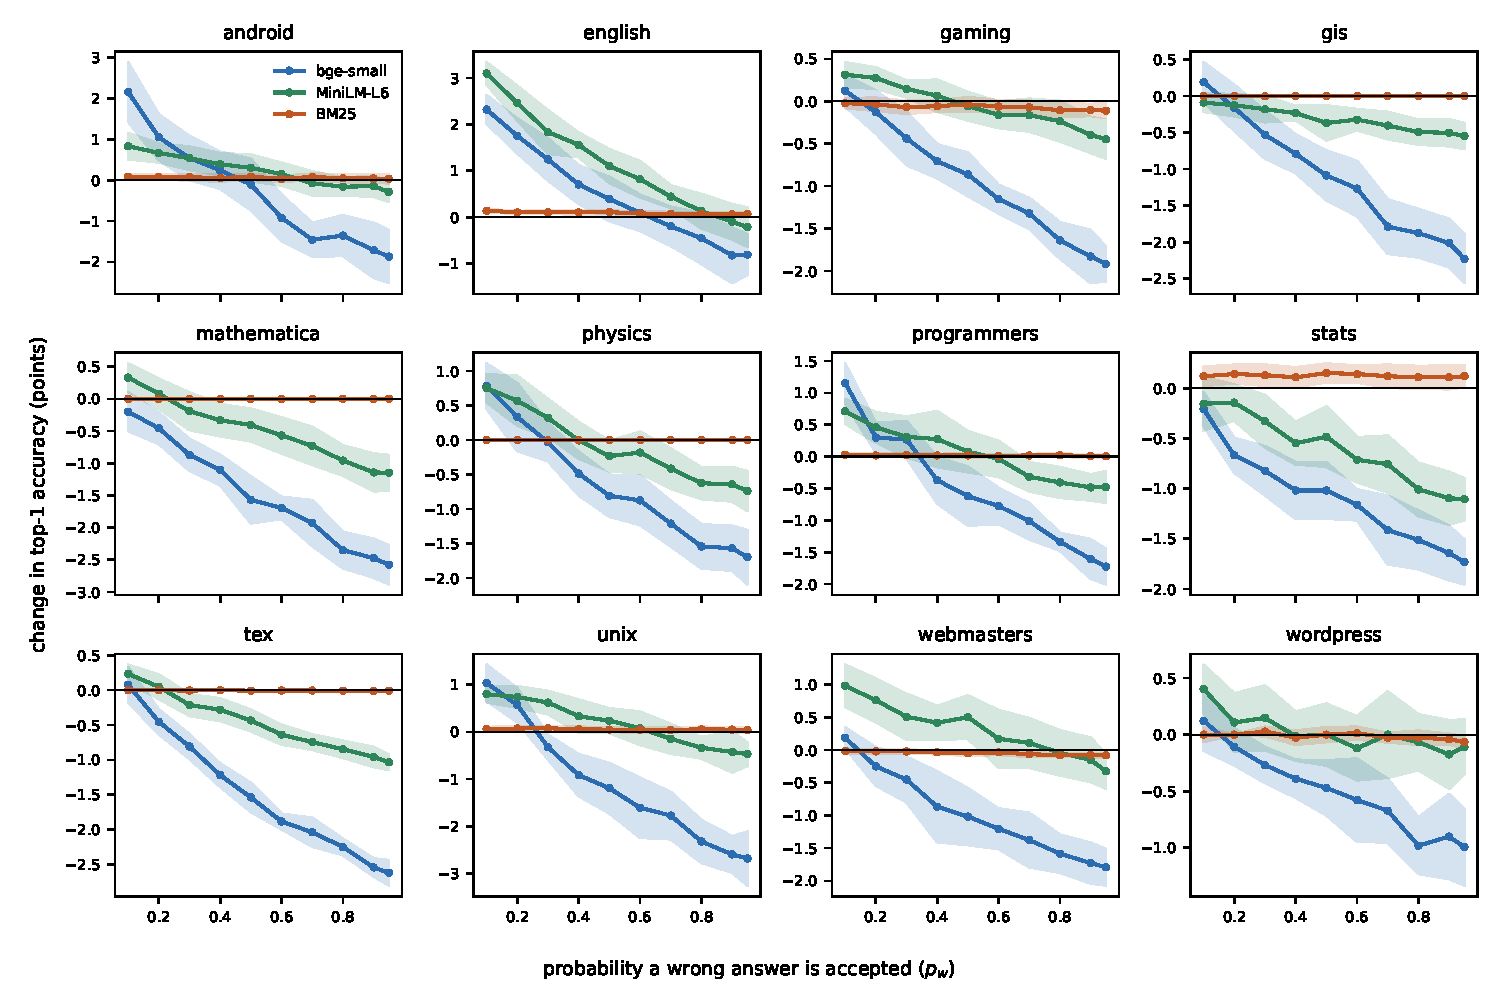
\includegraphics[width=\linewidth]{../figs/delta_r10_all.pdf}
\caption{Change in top-1 accuracy over the stream from naive write-back, relative to no write-back on the same order, as the acceptance rate of wrong answers grows. Bands are 95\% intervals over ten orders. Ten rounds.}
\label{fig:delta}
\end{figure}

\paragraph{The loop changes sign.} Figure~\ref{fig:delta} shows the paired change in top-1 accuracy for every forum and retriever. For both dense retrievers, the curve falls almost linearly with $p_w$ (median $R^2$ of a linear fit above 0.95). When users reject most wrong answers, write-back helps on most forums, by up to 3.1 points. When they accept nearly all of them, it hurts: at $p_w=0.95$ the change for dense retrievers ranges from \naiveMin{} to \naiveMax{} points, and the 95\% interval lies entirely below zero in \negNF{} of \nDense{} dense configurations. With base top-1 accuracies between 9\% and 35\% (Table~\ref{tab:cross}), a loss of 2.7 points is roughly a tenth of all correct answers. The pilot's numbers for Unix and Android are reproduced in direction and size (the pilot reported $-2.1$ and $-1.8$ points at $p_w=0.95$ with five orders; here $-2.68\pm0.57$ and $-1.87\pm0.65$ with ten orders, a re-computed embedding, and batch semantics that match the pilot).

\begin{table}[t]\centering\scriptsize
\begin{tabular}{llrrlll}\toprule Forum & Retriever & Top-1 & Hit@5 & Observed $p^*$ (top-1) & Observed $p^*$ (hit@5) & Plug-in $\hat p^*$\\\midrule
android & bge & 16.7 & 32.8 & 0.47 [0.37, 0.54] & 0.55 [0.39, 0.63] & 0.39\\
 & MiniLM & 22.3 & 38.9 & 0.67 [0.56, 0.78] & 0.67 [0.48, 0.89] & 0.69\\
 & BM25 & 13.7 & 23.0 & $>$0.95 & $>$0.95 & $>$0.95\\
\addlinespace[1pt]
english & bge & 19.1 & 34.2 & 0.63 [0.50, 0.75] & 0.39 [0.33, 0.44] & 0.61\\
 & MiniLM & 23.0 & 40.6 & 0.86 [0.77, 0.95] & 0.53 [0.46, 0.60] & 0.85\\
 & BM25 & 11.2 & 17.9 & $>$0.95 & 0.59 [0.37, 0.95] & $>$0.95\\
\addlinespace[1pt]
gaming & bge & 31.7 & 54.3 & 0.15 [0.10, 0.22] & $<$0.10 & 0.14\\
 & MiniLM & 34.7 & 57.0 & 0.45 [0.35, 0.56] & $<$0.10 & 0.49\\
 & BM25 & 27.0 & 41.1 & $<$0.10 & $<$0.10 & $<$0.10\\
\addlinespace[1pt]
gis & bge & 21.4 & 39.0 & 0.15 [0.10, 0.22] & 0.19 [0.16, 0.34] & 0.14\\
 & MiniLM & 25.2 & 44.4 & $<$0.10 & 0.31 [0.22, 0.41] & $<$0.10\\
 & BM25 & 16.8 & 29.9 & $>$0.95 & 0.10 [0.10, 0.40] & --\\
\addlinespace[1pt]
mathematica & bge & 12.1 & 26.1 & $<$0.10 & 0.12 [0.10, 0.19] & $<$0.10\\
 & MiniLM & 13.0 & 28.0 & 0.23 [0.17, 0.31] & 0.20 [0.15, 0.31] & 0.24\\
 & BM25 & 9.4 & 18.7 & $>$0.95 & $<$0.10 & --\\
\addlinespace[1pt]
physics & bge & 20.2 & 36.1 & 0.29 [0.19, 0.34] & 0.25 [0.18, 0.29] & 0.29\\
 & MiniLM & 21.5 & 40.4 & 0.40 [0.33, 0.47] & 0.28 [0.16, 0.37] & 0.45\\
 & BM25 & 13.5 & 24.3 & $>$0.95 & 0.20 [0.10, 0.40] & --\\
\addlinespace[1pt]
programmers & bge & 16.4 & 33.3 & 0.34 [0.30, 0.39] & 0.20 [0.17, 0.30] & 0.36\\
 & MiniLM & 17.4 & 34.3 & 0.57 [0.33, 0.66] & 0.56 [0.36, 0.73] & 0.47\\
 & BM25 & 11.6 & 20.1 & $>$0.95 & $<$0.10 & $>$0.95\\
\addlinespace[1pt]
stats & bge & 18.1 & 31.5 & $<$0.10 & 0.16 [0.11, 0.19] & $<$0.10\\
 & MiniLM & 20.2 & 35.7 & $<$0.10 & 0.35 [0.31, 0.41] & 0.11\\
 & BM25 & 15.8 & 24.9 & $>$0.95 & $>$0.95 & --\\
\addlinespace[1pt]
tex & bge & 11.5 & 22.7 & 0.11 [0.10, 0.14] & 0.14 [0.11, 0.16] & 0.13\\
 & MiniLM & 14.4 & 28.4 & 0.22 [0.16, 0.27] & 0.26 [0.21, 0.32] & 0.17\\
 & BM25 & 10.6 & 18.7 & 0.10 [0.10, 0.40] & $<$0.10 & $<$0.10\\
\addlinespace[1pt]
unix & bge & 20.8 & 36.3 & 0.26 [0.24, 0.29] & 0.28 [0.26, 0.31] & 0.24\\
 & MiniLM & 23.1 & 44.1 & 0.63 [0.50, 0.74] & 0.55 [0.45, 0.65] & 0.73\\
 & BM25 & 14.1 & 22.3 & $>$0.95 & $>$0.95 & $>$0.95\\
\addlinespace[1pt]
webmasters & bge & 10.8 & 21.1 & 0.14 [0.11, 0.19] & 0.16 [0.13, 0.19] & 0.16\\
 & MiniLM & 12.3 & 24.9 & 0.77 [0.56, 0.93] & 0.59 [0.50, 0.78] & 0.69\\
 & BM25 & 9.3 & 16.1 & $<$0.10 & 0.85 [0.57, 0.95] & $<$0.10\\
\addlinespace[1pt]
wordpress & bge & 14.0 & 27.8 & 0.15 [0.10, 0.20] & $<$0.10 & 0.13\\
 & MiniLM & 16.9 & 31.5 & 0.39 [0.17, 0.95] & $>$0.95 & 0.48\\
 & BM25 & 14.8 & 24.1 & 0.35 [0.10, 0.87] & 0.10 [0.10, 0.50] & 0.61\\
\bottomrule\end{tabular}
\caption{No-write-back accuracy (\%) and the crossover acceptance rate $p^*$ for naive write-back, with 95\% bootstrap intervals over ten orders. The last column is the plug-in prediction of Section~\ref{sec:model}, calibrated from the runs at $p_w=0.3$ only. ``--'': no entry ever changed an answer.}
\label{tab:cross}
\end{table}

\paragraph{The crossover is not a constant.} Table~\ref{tab:cross} lists $p^*$. Among dense configurations with an interior crossover it ranges from \crossMin{} to \crossMax{}. On some forums (stats, mathematica with bge, gis with MiniLM) write-back is harmful at every tested acceptance rate. The weaker MiniLM model often has a \emph{higher} crossover than bge on the same forum, so a better base retriever does not by itself make write-back safer. Crossovers for hit@5 are broadly similar but noisier. The intervals are wide in places (for example MiniLM on wordpress), because the curve is nearly flat there.

\paragraph{BM25 is nearly immune here.} With BM25, write-back changes accuracy by less than 0.2 points in every forum and condition, and written-back entries supply at most \ssBmMax\% of top-1 answers in the second half of the stream, against \ssMin--\ssMax\% for dense retrievers at $p_w=0.95$. The reason is visible before any simulation. For each ask we compare its score against the best original post with its score against the best other ask from the same family, as if that ask had been written back. Under bge, the other ask scores higher for 36--72\% of asks (depending on forum); under MiniLM for 20--49\%; under BM25 for only 2--12\%. Short titles share few terms with a new title and lose to long posts that match more terms. Dense encoders place two short titles close together whether or not they describe the same problem: under bge an ask from a \emph{different} family outscores the best original post for 33--74\% of asks. This is the mechanism of the takeover, and it also explains why most of the harm comes from wrong entries capturing questions they do not belong to. We do not claim BM25 is safe in general; with longer written-back entries (for example, the full generated answer) the picture may differ.

\begin{figure}[t]\centering
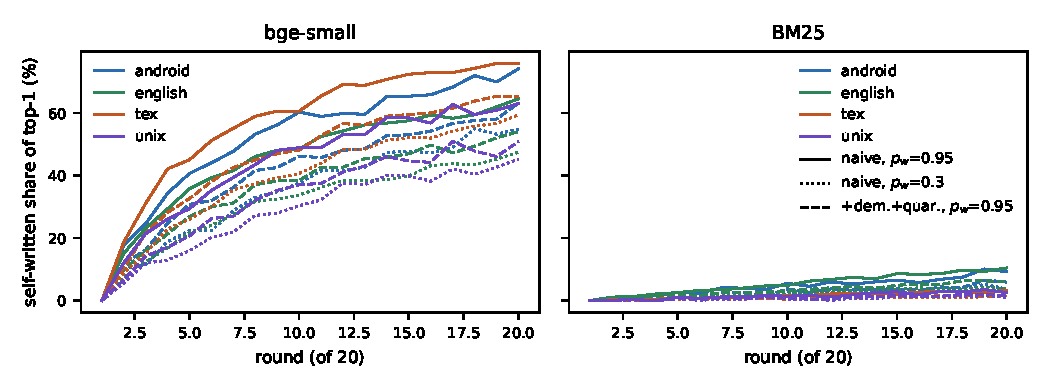
\includegraphics[width=0.85\linewidth]{../figs/selfshare_r20.pdf}
\caption{Share of top-1 answers that come from written-back entries over 20 rounds, averaged over ten orders. Left: bge-small. Right: BM25.}
\label{fig:selfshare}
\end{figure}

\paragraph{Self-written entries take over retrieval.} Figure~\ref{fig:selfshare} shows the takeover over 20 rounds. With bge and naive write-back at $p_w=0.95$, written-back entries supply more than half of all top-1 answers by round 9 to 13 (of 20) on all four forums, and 61--76\% by the end. Safeguards slow the takeover but do not stop it.

\paragraph{Longer streams.} Doubling the number of rounds to 20 on four forums leaves crossovers and losses within the intervals of the 10-round runs (Table~\ref{tab:r20}). The stream length in asks is the same; only the re-indexing interval is shorter. A longer stream of new asks would need more data than CQADupStack provides.

\begin{table}[t]\centering\scriptsize
\begin{tabular}{llllll}\toprule Forum & Retriever & $p^*$ (10 rounds) & $p^*$ (20 rounds) & Naive, $p_w{=}0.95$ (10) & (20)\\\midrule
android & bge & 0.47 [0.37, 0.54] & 0.45 [0.36, 0.53] & -1.87 $\pm$ 0.65 & -2.04 $\pm$ 0.69\\
 & MiniLM & 0.67 [0.56, 0.78] & 0.66 [0.55, 0.91] & -0.29 $\pm$ 0.24 & -0.29 $\pm$ 0.25\\
english & bge & 0.63 [0.50, 0.75] & 0.61 [0.50, 0.70] & -0.81 $\pm$ 0.44 & -0.84 $\pm$ 0.42\\
 & MiniLM & 0.86 [0.77, 0.95] & 0.82 [0.77, 0.95] & -0.21 $\pm$ 0.42 & -0.22 $\pm$ 0.48\\
tex & bge & 0.11 [0.10, 0.14] & 0.12 [0.10, 0.15] & -2.62 $\pm$ 0.18 & -2.73 $\pm$ 0.22\\
 & MiniLM & 0.22 [0.16, 0.27] & 0.22 [0.17, 0.27] & -1.03 $\pm$ 0.11 & -1.08 $\pm$ 0.10\\
unix & bge & 0.26 [0.24, 0.29] & 0.26 [0.22, 0.28] & -2.68 $\pm$ 0.57 & -2.95 $\pm$ 0.57\\
 & MiniLM & 0.63 [0.50, 0.74] & 0.63 [0.51, 0.77] & -0.47 $\pm$ 0.24 & -0.47 $\pm$ 0.32\\
\bottomrule\end{tabular}
\caption{Crossover and loss at $p_w=0.95$ with 10 and 20 rounds on four forums.}
\label{tab:r20}
\end{table}

\paragraph{Safeguards recover part of the loss.} Table~\ref{tab:safe} (Appendix~\ref{app:safe}) reports the paired change at $p_w=0.3$ and $0.95$ for the dense retrievers. At $p_w=0.3$, write-back with demotion and quarantine is positive in \rqPosThree{} of \nDense{} dense configurations. At $p_w=0.95$ it turns the loss into a non-negative change in \rqTurned{} of \nDense{} configurations. In the other \nStill{} it recovers a median of \recMedStill\% of the loss (range \recMinStill--\recMaxStill\%), so the loss is reduced but not removed. Quarantine adds very little on top of demotion: the two differ by at most \qDiffMax{} points at $p_w=0.95$. With a 90\% acceptance rate for correct answers, few entries are rejected twice before they have done their damage.


\section{What the stored entry contains}
\label{sec:ablation}
\begin{table}[t]\centering\scriptsize
\resizebox{\linewidth}{!}{\begin{tabular}{llrrrrrrr}\toprule Retriever & Entry content & $\Delta$ @0.3 & $\Delta$ @0.95 & sig.\ $<0$ @0.95 & median $p^*$ & self-share @0.95 & capture & steal\\\midrule
bge & ask text (v1) & -0.21 & -1.89 & 12/12 & 0.15 & 56\% & 74\% & 26.3\%\\
 & shown thread text & +0.00 & +0.00 & 0/12 & $>$0.95 & 0\% & 51\% & 0.0\%\\
 & ask + thread text & +0.14 & -0.02 & 1/12 & 0.75 & 14\% & 52\% & 2.7\%\\
\addlinespace[2pt]
MiniLM & ask text (v1) & +0.29 & -0.58 & 10/12 & 0.43 & 33\% & 58\% & 12.2\%\\
 & shown thread text & +0.00 & +0.00 & 0/12 & $>$0.95 & 0\% & 47\% & 0.0\%\\
 & ask + thread text & +0.20 & -0.02 & 4/12 & 0.80 & 18\% & 53\% & 3.5\%\\
\addlinespace[2pt]
BM25 & ask text (v1) & +0.03 & -0.00 & 4/12 & $>$0.95 & 4\% & 30\% & 0.6\%\\
 & shown thread text & +0.00 & +0.00 & 0/12 & $>$0.95 & 0\% & 47\% & 0.0\%\\
 & ask + thread text & +0.07 & +0.01 & 2/12 & $>$0.95 & 13\% & 52\% & 1.6\%\\
\bottomrule\end{tabular}}
\caption{Entry-content ablation, naive write-back. $\Delta$: mean over the twelve forums of the paired change in top-1 accuracy (points) at $p_w=0.3$ and $0.95$. ``sig.\ $<0$'': forums whose 95\% interval at $p_w=0.95$ is below zero. Median $p^*$ over forums (crossovers below or above the grid counted at the grid ends). Self-share: share of top-1 answers from written-back entries, second half of the stream. Capture and steal: see Section~\ref{sec:setup}.}
\label{tab:ablation}
\end{table}
\begin{figure}[t]\centering
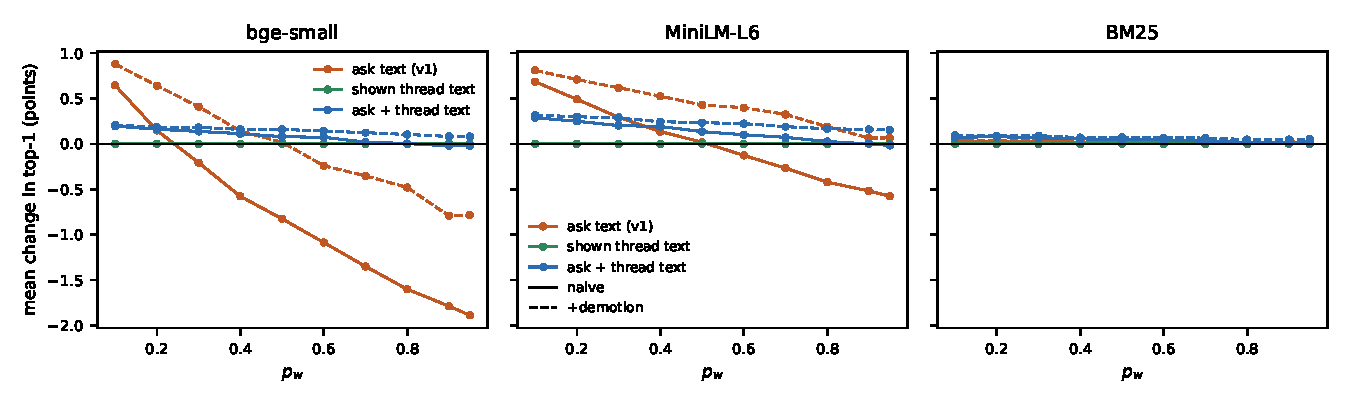
\includegraphics[width=\linewidth]{../figs/ablation_v2.pdf}
\caption{Mean paired change in top-1 accuracy over the twelve forums for the three entry contents, naive (solid) and with demotion (dashed).}
\label{fig:ablation}
\end{figure}

Version 1 stored the ask text. Table~\ref{tab:ablation} and Figure~\ref{fig:ablation} compare the three entry contents; per-configuration crossovers are in Table~\ref{tab:ablcross} (Appendix).

\paragraph{Question entries steal answers.} With question entries and bge, a wrong entry scores above the canonical post on \stealBgeAsk\% of the asks that the base retriever answers correctly (MiniLM \stealMiniAsk\%, BM25 \stealBmAsk\%). That is the harm channel: the incoming question is a short title, and another short title, even about a different problem, is closer to it than any full post. The ordering of retrievers by steal rate matches their ordering by harm.

\paragraph{Thread copies are inert for top-1.} A copy of the shown thread scores exactly like the original post, so it can never rank above it, and the top-1 thread never changes: the change in top-1 accuracy is zero by construction at every $p_w$. Capture is still about half, but only because copies of a wrong post that already outranked the canonical one inherit its score; steal is zero. Copies do crowd the top five: hit@5 falls by 1.2 points on average at $p_w=0.95$ for both dense retrievers. This variant gives neither the gain nor the loss of write-back.

\paragraph{Question plus thread text keeps a little of the gain and little of the loss.} Concatenating the ask with the thread text puts the entry between a question and a post. Steal falls to \stealBgeAskdoc\% (bge) and \stealMiniAskdoc\% (MiniLM). The mean change at $p_w=0.95$ moves from \dNNBgeAsk{} to \dNNBgeAskdoc{} points for bge and from \dNNMiniAsk{} to \dNNMiniAskdoc{} for MiniLM; the loss is significant in \negBgeAskdoc{} (bge) and \negMiniAskdoc{} (MiniLM) of twelve forums instead of \negBgeAsk{} and \negMiniAsk{}. The median crossover rises from \medBgeAsk{} to \medBgeAskdoc{} (bge) and from \medMiniAsk{} to \medMiniAskdoc{} (MiniLM). The gain at low $p_w$ also shrinks: at $p_w=0.1$ the mean change falls from 0.64 to 0.20 points (bge) and from 0.68 to 0.29 (MiniLM), and the largest single-forum gain from 2.3 to 0.6 (bge) and 3.1 to 1.0 points (MiniLM). The curve is flatter rather than shifted: at $p_w=0.3$ the concatenated entries do better than question entries for bge (\dThBgeAskdoc{} against \dThBgeAsk) and slightly worse for MiniLM (\dThMiniAskdoc{} against \dThMiniAsk). With demotion the concatenated entries are non-negative on average across the grid. BM25 stays essentially unaffected with all three entry types, including the longer concatenated entries that v1 flagged as untested.

The trade-off is the point. The same property that makes a stored question useful, that it looks like the next question, is what lets a wrong one capture answers. Entry designs that reduce one reduce the other. In this data no design gave the full gain of question entries without their loss.

\paragraph{A cross-encoder reranker.} We tried to raise base accuracy with a cross-encoder over the bge candidates (Table~\ref{tab:ce}). It did not: top-1 accuracy changed by \ceGainMin{} to \ceGainMax{} points (the reranker is trained on web queries and passages, not forum titles). It did change the loop. Reranked, written-back questions supply 6--19\% of top-1 answers at $p_w=0.95$ instead of 56--72\%, and the change at $p_w=0.95$ lies between $-0.13$ and $+0.24$ points (significantly negative on \ceNeg{} of \ceN{} forums, mathematica), against $-1.8$ to $-2.7$ for bge alone. The steal rate falls from 30--39\% under bge to at most 1.1\% after reranking: the cross-encoder does not give a wrong stored title the advantage over the correct post that the bi-encoder does. Because base accuracy did not rise, this run does not tell us whether the effect holds at higher base accuracy; that question remains open.

\begin{table}[t]\centering\scriptsize
\begin{tabular}{llrrlll}\toprule Forum & Retriever & Top-1 & Hit@5 & $p^*$ & $\Delta$@0.95 & self-share @0.95\\\midrule
android & bge & 16.7 & 32.8 & 0.47 [0.37, 0.54] & -1.87 $\pm$ 0.65 & 65\%\\
 & bge+CE & 17.6 & 31.4 & $>$0.95 & +0.24 $\pm$ 0.12 & 10\%\\
mathematica & bge & 12.1 & 26.1 & $<$0.10 & -2.58 $\pm$ 0.30 & 65\%\\
 & bge+CE & 12.3 & 25.5 & 0.73 [0.29, 0.93] & -0.13 $\pm$ 0.11 & 7\%\\
unix & bge & 20.8 & 36.3 & 0.26 [0.24, 0.29] & -2.68 $\pm$ 0.57 & 56\%\\
 & bge+CE & 20.0 & 34.0 & $>$0.95 & +0.18 $\pm$ 0.14 & 6\%\\
webmasters & bge & 10.8 & 21.1 & 0.14 [0.12, 0.19] & -1.79 $\pm$ 0.28 & 72\%\\
 & bge+CE & 11.7 & 20.4 & 0.81 [0.19, 0.95] & -0.02 $\pm$ 0.15 & 19\%\\
\bottomrule\end{tabular}
\caption{bge alone and bge with cross-encoder reranking (top 20), question entries, naive write-back. Self-share in the second half of the stream.}
\label{tab:ce}
\end{table}

\section{Acceptance that depends on confidence}
\label{sec:difficulty}
If users accept wrong answers more readily when the system is confident, the accepted wrong answers are concentrated on asks where the retriever is confidently wrong, and these are the asks whose entries are most likely to resemble future asks. Table~\ref{tab:diff} (Appendix) and Figure~\ref{fig:diff} compare crossovers under constant and confidence-dependent acceptance with the same average rate. For question entries and dense retrievers, the crossover moves down in most configurations (median shift \diffMedShift, range \diffMinShift{} to \diffMaxShift); each crossover lies outside the other's bootstrap interval, or censoring changes, downwards in \diffDown{} of \nDenseV{} configurations and upwards in \diffUp. The mean loss at $p_w=0.95$ is nearly unchanged (\diffDnnConst{} versus \diffDnnDiff{} points) because at that rate almost all wrong answers are accepted either way. The qualitative picture of Section~\ref{sec:results} holds; crossovers measured under constant acceptance are, if anything, slightly optimistic.

\begin{figure}[t]\centering
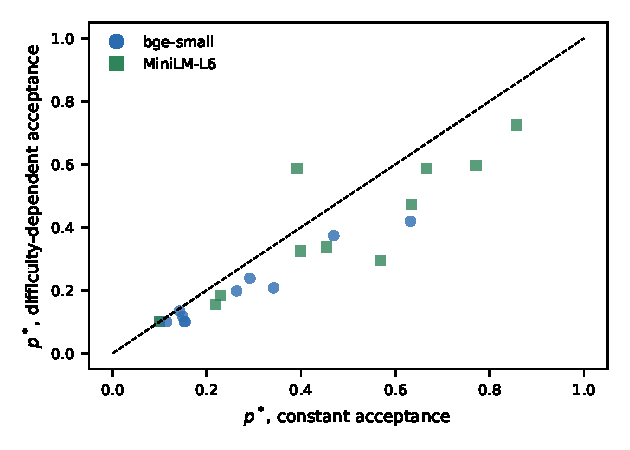
\includegraphics[width=0.5\linewidth]{../figs/difficulty_v2.pdf}
\caption{Crossover under constant against confidence-dependent acceptance of wrong answers, question entries, dense retrievers. Points at 0.05 and 1.0 are below or above the grid.}
\label{fig:diff}
\end{figure}

\section{Safeguards and baselines}
\label{sec:baselines}
\begin{table}[t]\centering\scriptsize
\begin{tabular}{llrrrrrr}\toprule Entry content & Rule & $\Delta$@0.3 & $\Delta$@0.6 & $\Delta$@0.8 & $\Delta$@0.95 & $\ge0$ @0.95 & entries kept\\\midrule
ask text (v1) & naive & +0.04 & -0.61 & -1.01 & -1.23 & 0/24 & 100\%\\
 & +demotion & +0.51 & +0.08 & -0.15 & -0.36 & 9/24 & 100\%\\
 & +dem.+quar. & +0.65 & +0.17 & -0.13 & -0.37 & 9/24 & 100\%\\
 & confidence gate & +0.16 & -0.34 & -0.67 & -0.83 & 2/24 & 63\%\\
 & footprint rule & -0.04 & -0.59 & -0.93 & -1.09 & 0/24 & 79\%\\
\addlinespace[2pt]
shown thread text & naive & +0.00 & +0.00 & +0.00 & +0.00 & 24/24 & 100\%\\
 & +demotion & +0.00 & +0.00 & +0.00 & +0.00 & 24/24 & 100\%\\
 & +dem.+quar. & +0.05 & +0.02 & +0.00 & -0.00 & 16/24 & 100\%\\
 & confidence gate & +0.00 & +0.00 & +0.00 & +0.00 & 24/24 & 55\%\\
 & footprint rule & +0.00 & +0.00 & +0.00 & +0.00 & 24/24 & 85\%\\
\addlinespace[2pt]
ask + thread text & naive & +0.17 & +0.09 & +0.02 & -0.02 & 7/24 & 100\%\\
 & +demotion & +0.23 & +0.18 & +0.14 & +0.12 & 20/24 & 100\%\\
 & +dem.+quar. & +0.29 & +0.21 & +0.14 & +0.11 & 20/24 & 100\%\\
 & confidence gate & +0.14 & +0.08 & +0.04 & +0.02 & 14/24 & 56\%\\
 & footprint rule & +0.13 & +0.05 & -0.01 & -0.04 & 8/24 & 90\%\\
\bottomrule\end{tabular}
\caption{Mean paired change in top-1 accuracy over the \nDenseV{} dense configurations for each entry content and safeguard. ``$\ge0$'': configurations with a non-negative mean change at $p_w=0.95$. Entries kept: written-back entries at the end of the stream relative to naive, at $p_w=0.95$.}
\label{tab:baselines}
\end{table}

Table~\ref{tab:baselines} compares the v1 safeguards with the two new baselines. For question entries, demotion is the strongest: at $p_w=0.95$ it reduces the mean loss from \blAskNaive{} to \blAskDem{} points and is non-negative in \blNNAskDem{} of \nDenseV{} configurations; quarantine adds little (\blAskQuar). The confidence gate keeps \blKeptAskGate\% of the entries and reduces the loss to \blAskGate{} points, with smaller gains at low $p_w$ (\blThAskGate{} at 0.3, against \blThAskDem{} for demotion). The footprint rule keeps \blKeptAskFoot\% of the entries and barely changes the outcome (\blAskFoot{} at 0.95, \blThAskFoot{} at 0.3): it removes entries that resemble existing entries for the same thread, whether those entries are right or wrong, so it does not target the entries that cause harm. Both rules use only signals available without labels, but neither targets wrong entries; demotion does, through the user who reopens. With question-plus-thread entries every rule is close to zero, and demotion again does best (\blAskdocDem{} at 0.95, non-negative in \blNNAskdocDem{} of \nDenseV).

\section{A model of the crossover}
\label{sec:model}
\paragraph{An exact decomposition.} Under naive write-back no original post is ever withdrawn, so an answer can differ from the no-write-back answer only when the top-1 result is a written-back entry. Attributing each such change to the entry that caused it gives an exact identity
\begin{equation}
N\,\Delta = C\,\bar e_c + W\,\bar e_w,
\label{eq:decomp}
\end{equation}
where $N$ is the number of asks, $\Delta$ the change in accuracy, $C$ and $W$ the numbers of correct and wrong entries that were written and became retrievable, and $\bar e_c$ and $\bar e_w$ the average net number of answers each kind of entry turned from wrong to right (minus right to wrong). We count these quantities directly in the simulation.

\paragraph{First-order approximation.} If the system's accuracy on the asks that generate entries stays near its no-write-back accuracy $A$, then $C\approx p_c A N'$ and $W\approx p_w(1-A)N'$, with $N'$ the number of asks whose entries become retrievable. If the per-entry effects do not depend on $p_w$, setting $\Delta=0$ gives
\begin{equation}
p^* \approx \frac{p_c\,A}{1-A}\cdot\frac{\bar e_c}{-\bar e_w}.
\label{eq:pstar}
\end{equation}
Both assumptions are approximations: entries compete with each other, so per-entry effects shrink as more entries are written, and write-back itself changes the accuracy of later asks.

\paragraph{A one-parameter law does not fit.} If the ratio $\kappa=\bar e_c/(-\bar e_w)$ were the same everywhere, $p^*$ would be a function of base accuracy alone. Fitting a single $\kappa$ by least squares to the \nOne{} interior crossovers gives $\kappa=\kappaOne$ but $R^2=\rsqOne$ (Spearman $\rho=\rhoOne$; Figure~\ref{fig:cross}a). Base accuracy alone does not predict when write-back becomes harmful. Gaming has the highest base accuracy and one of the lowest crossovers for bge.

\paragraph{A plug-in estimate does.} The ratio $\kappa$ is specific to the forum and retriever: in our runs $\bar e_c$ ranges from about zero to $0.15$ answers gained per correct entry, while $\bar e_w$ lies between $-0.01$ and $-0.08$ (dense retrievers, $p_w=0.3$). Measuring $\bar e_c$ and $\bar e_w$ from the runs at a single acceptance rate ($p_w=0.3$) and inserting them into Eq.~\eqref{eq:pstar} predicts the crossover found from the full sweep with mean absolute error \plugMAE{} and Spearman $\rho=\plugRho$ over the \plugN{} configurations where both are interior. Prediction and observation agree, within the bootstrap interval ($\pm0.05$) or in the direction of censoring, for \plugAgree{} of \plugTot{} configurations where the estimate is defined (Figure~\ref{fig:cross}b, Table~\ref{tab:cross}). Calibrating at $p_w=0.5$ or $0.95$ instead gives mean absolute errors of \plugMAEfive{} and \plugMAEnn{}. \paragraph{Out of sample.} The calibration above uses the same orders as the sweep it predicts. We therefore split the ten orders into two halves, estimate $\bar e_c$ and $\bar e_w$ at $p_w=0.3$ on one half, and compare the prediction with the crossover observed on the other half, in both directions (all 36 configurations plus the four reranker configurations). Over the \oosNAskTh{} cases where both are interior, the mean absolute error is \oosMAEAskTh{} and Spearman $\rho=\oosRhoAskTh$; prediction and observation fall in the same class (below, inside or above the grid) in \oosSameAskTh{} of \oosDefAskTh{} cases where the estimate is defined. Calibrating at $p_w=0.5$ gives \oosMAEAskFi{} ($\rho=\oosRhoAskFi$). The out-of-sample error is larger than the in-sample \plugMAE{} of version 1 but the ranking is preserved. For question-plus-thread entries the estimate fails (MAE \oosMAEAskdocTh, $\rho=\oosRhoAskdocTh$): the per-entry effects are close to zero and too noisy to estimate from five orders, and the crossover itself is poorly determined because the curve is nearly flat.

This is an empirical check of a first-order model, not a proof. It does have a practical reading. The per-entry effects can be estimated in deployment from a small audited sample of written-back entries, and the deployment's own acceptance rate for wrong answers can then be compared against the predicted $p^*$.

\begin{figure}[t]\centering
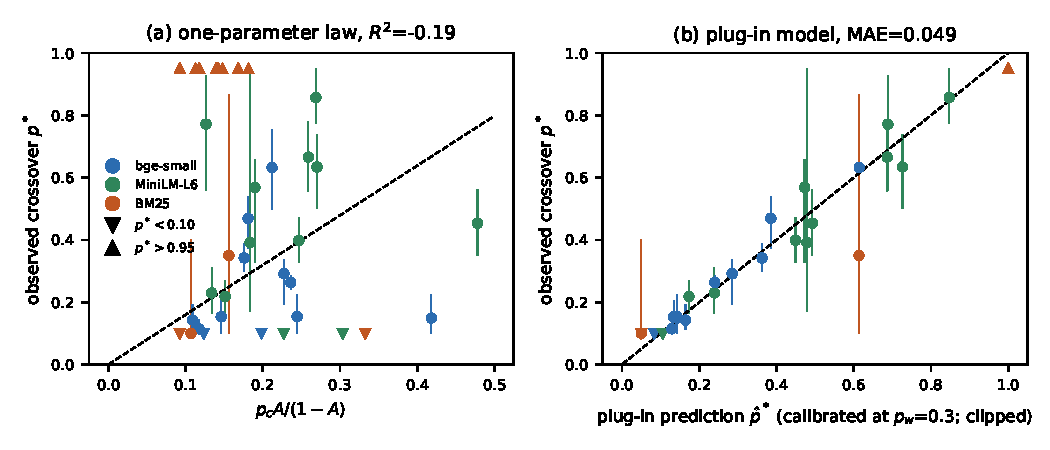
\includegraphics[width=\linewidth]{../figs/crossover_two.pdf}
\caption{Observed crossover against (a) the one-parameter law $p^*=\kappa\,p_cA/(1-A)$ and (b) the plug-in estimate of Eq.~\eqref{eq:pstar} calibrated at $p_w=0.3$. Triangles mark crossovers outside the tested grid; bars are 95\% bootstrap intervals.}
\label{fig:cross}
\end{figure}

\section{Monitoring without labels}
\label{sec:monitor}
In deployment the true error is unknown. The pilot tested one label-free signal and it failed. Here we test five, all computed without ground truth:
(i) the \emph{acceptance rate}, which any deployment observes and which serves as a baseline;
(ii) the \emph{self-written share} of top-1 answers;
(iii) the pilot's signal, the share of answers where a written-back entry wins and the best original post points to a different thread;
(iv) \emph{disagreement with an independent retriever}, the share of asks whose deployed top-1 thread differs from that of a static retriever of a different kind (BM25 for dense deployments, bge for BM25), together with its rise since round 1;
(v) \emph{probe-bank drift}, the share of a fixed bank of 200 asks, queried read-only after each round, whose top-1 thread has changed since the start.

For each forum and retriever, a run (one condition, acceptance rate and order) is labelled harmful if its accuracy over the second half of the stream is below no write-back on the same order. We report the Spearman correlation between each signal (averaged over the second half) and the true accuracy change, pooled over all runs and within a fixed $p_w$, and the AUROC for harmful runs using the signal value at a given round. All values are averaged over the 36 forum--retriever pairs (Table~\ref{tab:monitor}, Figure~\ref{fig:monitor}).

\begin{table}[t]\centering\small
\resizebox{\linewidth}{!}{\begin{tabular}{lrrrrr}\toprule Signal & $\rho$ (all runs) & $\rho$ (fixed $p_w$) & AUROC r2 & AUROC r5 & AUROC r10\\\midrule
Acceptance rate (baseline) & -0.41 & +0.06 & 0.70 & 0.70 & 0.70\\
Self-written share of top-1 & -0.51 & -0.34 & 0.69 & 0.73 & 0.73\\
Pilot signal: self vs.\ human top entry & -0.51 & -0.34 & 0.67 & 0.74 & 0.73\\
Disagreement with independent retriever & -0.32 & -0.21 & 0.54 & 0.58 & 0.60\\
\quad rise since round 1 & -0.13 & -0.07 & 0.54 & 0.57 & 0.58\\
Probe-bank drift & -0.44 & -0.29 & 0.71 & 0.76 & 0.77\\
\bottomrule\end{tabular}}
\caption{Label-free signals against the true change in accuracy. $\rho$: Spearman correlation with the accuracy change (negative means the signal rises as accuracy falls), averaged over forum--retriever pairs. AUROC for identifying harmful runs from the signal after round 2, 5 and 10. Ten rounds.}
\label{tab:monitor}
\end{table}

\begin{figure}[t]\centering
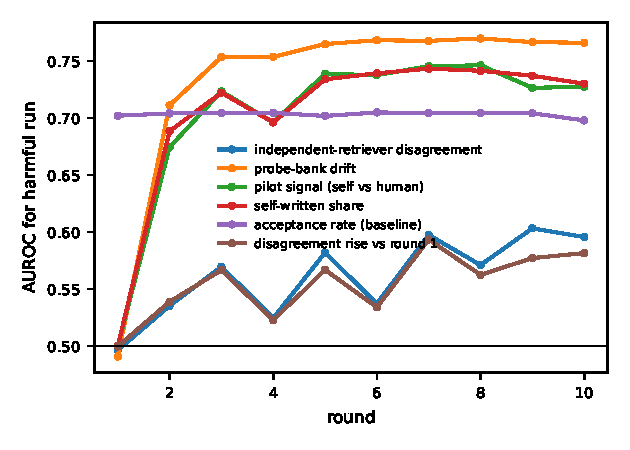
\includegraphics[width=0.55\linewidth]{../figs/monitor_r10_all.pdf}
\caption{AUROC for identifying harmful runs from each label-free signal, by round.}
\label{fig:monitor}
\end{figure}

\paragraph{Results.} The acceptance rate alone gives an AUROC of about 0.70 from the first round, because harm is driven mostly by how often wrong answers are accepted. The self-written share, the pilot signal and probe-bank drift reach 0.72--0.77 after three to five rounds, a small gain over the baseline that arrives late. Within a fixed acceptance rate their correlation with the true accuracy change is weak ($|\rho|\le0.34$). Disagreement with an independent retriever is close to chance (AUROC 0.50--0.61), and its rise since round 1 even more so. The reason is that dense and lexical retrievers already disagree on most asks before any write-back: under bge and BM25 the top-1 thread differs for about 80\% of Android asks. Changes caused by the loop are small against that background. In summary, none of these monitors detects harm in a way that adds much to the acceptance rate. The independent-retriever monitor, which we expected to work best because it does not share the deployed retriever's errors, did not.

\section{Limitations}
\textbf{Simulated acceptance.} User acceptance is the only simulated component, and it is the one that matters most. Real acceptance probably depends on the question, the answer and the user, and acceptance of wrong answers is likely correlated with how plausible they look. Version 2 adds one confidence-dependent acceptance model, which moves crossovers slightly down; real acceptance may depend on other things, such as answer length or user expertise. The plug-in model would still apply if the per-entry effects were measured under the real acceptance process, but the crossovers reported here would not.
\textbf{Incomplete ground truth.} CQADupStack duplicate links are incomplete \citep{hoogeveen2015cqadupstack}: an answer we count as wrong may in fact solve the problem. This affects absolute accuracies and could make some ``wrong'' entries harmless, which would raise $p^*$.
\textbf{Short questions.} Asks are post titles, which makes retrieval hard (base top-1 accuracy 9--35\%) and makes written-back entries short. Storing the ask with the thread text removes most of the effect (Section~\ref{sec:ablation}); entries containing a generated answer were not tested. The cross-encoder did not raise base accuracy, so whether the loop behaves the same at much higher base accuracy is open.
\textbf{Simplified write-back.} Entries point to an existing thread; there is no generation step, so we do not measure errors introduced by an LLM writing the answer. BM25 statistics are not updated as entries are added. The probe bank is drawn from the stream itself.
\textbf{Scope of the model.} The model is first order and is checked on the same simulated data it describes. The out-of-sample test splits orders, not forums or data, so it is a weak form of out-of-sample evidence. The confidence gate and footprint thresholds were set by simple rules, not tuned; tuned versions may do better.

\section{Conclusion}
On real repeat questions from twelve forums, writing accepted questions back into a dense retriever's knowledge base helps only while users reject most wrong answers. Version 2 shows that this is mostly a property of what is stored: a stored question wins because it resembles the next question, and storing it with the thread text, or reranking with a cross-encoder, removes most of the loss together with most of the gain. The acceptance rate at which it starts to hurt varies from below 0.10 to about 0.86 and is not predicted by base accuracy. It is predicted well by a first-order formula once the per-entry effects of correct and wrong entries are measured, and those effects can be estimated from a small audit. Reopening wrong answers reduces the loss but does not remove it, and the label-free monitors we tried add little to the acceptance rate. For practitioners: decide what an entry contains before deciding how to police it, prefer reopening of wrong answers over confidence or redundancy filters, and note that the most useful quantities to measure before turning on write-back are the acceptance rate of wrong answers and the per-entry effect of a wrong entry. Monitoring that works without labels remains an open problem.

\section*{Code and data availability}
All data are public (CQADupStack via the BEIR/MTEB distribution on Hugging Face). The code for data preparation, simulation and analysis, the cached per-run results and the scripts that generate every table and figure in this paper will be released on GitHub. Every number in the paper is produced by these scripts from saved runs. The full v1 experiment (embedding twelve forums with two dense models and 9{,}120 simulation runs) runs on a laptop in well under an hour; the version-2 additions (prep\_v2.py, sim\_v2.py, analyze\_v2.py) add about an hour, most of it cross-encoder scoring and the iterated embedding of concatenated entries.

\section*{Acknowledgements}
This work uses no employer or customer data. The retrieval setup follows TicketIQ, the author's M.Tech dissertation system.

\section*{Changes from version 1}
\begin{itemize}
\item Related work now covers generated content in retrieval corpora \citep{chen2024spiral,dai2024sourcebias,yu2026collapse,druck2026ragcollapse} and case-based reasoning \citep{aamodt1994cbr,smyth1995forget,zhu1999add}; the abstract and introduction describe the setting as the retrieval half of RAG.
\item New: entry-content ablation and capture/steal diagnostics (Section~\ref{sec:ablation}); confidence-dependent acceptance (Section~\ref{sec:difficulty}); confidence-gate and footprint baselines (Section~\ref{sec:baselines}); out-of-sample test of the plug-in estimate (Section~\ref{sec:model}); cross-encoder reranker on four forums.
\item Changed claims: the harm reported in v1 is specific to storing question text; it largely disappears with question-plus-thread entries or a cross-encoder reranker. The plug-in estimate's error is about \oosMAEAskTh{} out of sample rather than \plugMAE{} in sample. All v1 numbers for question entries are reproduced exactly by the v2 code.
\end{itemize}

\bibliography{refs}

\appendix
\section{Full safeguard results}\label{app:safe}
\begin{table}[h]\centering\scriptsize
\begin{tabular}{llrlll}\toprule Forum & Retriever & $p_w$ & Naive & + demotion & + demotion + quarantine\\\midrule
android & bge & 0.3 & +0.54 $\pm$ 0.53 & +1.79 $\pm$ 0.67 & +2.46 $\pm$ 0.90\\
 &  & 0.95 & -1.87 $\pm$ 0.65 & -0.43 $\pm$ 0.67 & -0.44 $\pm$ 0.72\\
 & MiniLM & 0.3 & +0.54 $\pm$ 0.28 & +0.92 $\pm$ 0.20 & +0.84 $\pm$ 0.36\\
 &  & 0.95 & -0.29 $\pm$ 0.24 & +0.31 $\pm$ 0.23 & +0.30 $\pm$ 0.26\\
\addlinespace[1pt]
english & bge & 0.3 & +1.25 $\pm$ 0.45 & +1.95 $\pm$ 0.38 & +2.16 $\pm$ 0.49\\
 &  & 0.95 & -0.81 $\pm$ 0.44 & +0.64 $\pm$ 0.36 & +0.61 $\pm$ 0.37\\
 & MiniLM & 0.3 & +1.84 $\pm$ 0.46 & +2.83 $\pm$ 0.26 & +2.85 $\pm$ 0.47\\
 &  & 0.95 & -0.21 $\pm$ 0.42 & +1.44 $\pm$ 0.28 & +1.34 $\pm$ 0.26\\
\addlinespace[1pt]
gaming & bge & 0.3 & -0.44 $\pm$ 0.31 & -0.05 $\pm$ 0.26 & +0.35 $\pm$ 0.28\\
 &  & 0.95 & -1.92 $\pm$ 0.20 & -0.92 $\pm$ 0.22 & -0.93 $\pm$ 0.23\\
 & MiniLM & 0.3 & +0.15 $\pm$ 0.10 & +0.39 $\pm$ 0.12 & +0.67 $\pm$ 0.19\\
 &  & 0.95 & -0.45 $\pm$ 0.23 & +0.03 $\pm$ 0.20 & +0.03 $\pm$ 0.21\\
\addlinespace[1pt]
gis & bge & 0.3 & -0.53 $\pm$ 0.32 & +0.06 $\pm$ 0.27 & +0.02 $\pm$ 0.27\\
 &  & 0.95 & -2.23 $\pm$ 0.33 & -1.08 $\pm$ 0.24 & -1.11 $\pm$ 0.27\\
 & MiniLM & 0.3 & -0.18 $\pm$ 0.18 & -0.07 $\pm$ 0.13 & -0.08 $\pm$ 0.13\\
 &  & 0.95 & -0.55 $\pm$ 0.18 & -0.30 $\pm$ 0.15 & -0.30 $\pm$ 0.15\\
\addlinespace[1pt]
mathematica & bge & 0.3 & -0.87 $\pm$ 0.24 & -0.30 $\pm$ 0.30 & -0.23 $\pm$ 0.30\\
 &  & 0.95 & -2.58 $\pm$ 0.30 & -1.41 $\pm$ 0.31 & -1.41 $\pm$ 0.31\\
 & MiniLM & 0.3 & -0.19 $\pm$ 0.29 & +0.40 $\pm$ 0.26 & +0.29 $\pm$ 0.29\\
 &  & 0.95 & -1.15 $\pm$ 0.27 & -0.42 $\pm$ 0.22 & -0.43 $\pm$ 0.21\\
\addlinespace[1pt]
physics & bge & 0.3 & -0.03 $\pm$ 0.28 & +0.56 $\pm$ 0.34 & +0.59 $\pm$ 0.32\\
 &  & 0.95 & -1.70 $\pm$ 0.39 & -0.72 $\pm$ 0.32 & -0.73 $\pm$ 0.32\\
 & MiniLM & 0.3 & +0.32 $\pm$ 0.27 & +0.64 $\pm$ 0.21 & +0.72 $\pm$ 0.16\\
 &  & 0.95 & -0.74 $\pm$ 0.29 & +0.04 $\pm$ 0.32 & +0.03 $\pm$ 0.32\\
\addlinespace[1pt]
programmers & bge & 0.3 & +0.27 $\pm$ 0.29 & +0.88 $\pm$ 0.25 & +1.00 $\pm$ 0.15\\
 &  & 0.95 & -1.73 $\pm$ 0.28 & -0.42 $\pm$ 0.27 & -0.41 $\pm$ 0.27\\
 & MiniLM & 0.3 & +0.31 $\pm$ 0.31 & +0.60 $\pm$ 0.27 & +0.51 $\pm$ 0.28\\
 &  & 0.95 & -0.48 $\pm$ 0.24 & +0.07 $\pm$ 0.31 & +0.07 $\pm$ 0.31\\
\addlinespace[1pt]
stats & bge & 0.3 & -0.82 $\pm$ 0.24 & -0.35 $\pm$ 0.15 & -0.19 $\pm$ 0.17\\
 &  & 0.95 & -1.73 $\pm$ 0.22 & -1.18 $\pm$ 0.24 & -1.18 $\pm$ 0.24\\
 & MiniLM & 0.3 & -0.33 $\pm$ 0.26 & -0.19 $\pm$ 0.24 & -0.22 $\pm$ 0.21\\
 &  & 0.95 & -1.11 $\pm$ 0.21 & -0.56 $\pm$ 0.30 & -0.57 $\pm$ 0.29\\
\addlinespace[1pt]
tex & bge & 0.3 & -0.81 $\pm$ 0.17 & -0.25 $\pm$ 0.24 & +0.13 $\pm$ 0.38\\
 &  & 0.95 & -2.62 $\pm$ 0.18 & -1.49 $\pm$ 0.23 & -1.49 $\pm$ 0.24\\
 & MiniLM & 0.3 & -0.21 $\pm$ 0.15 & +0.13 $\pm$ 0.15 & +0.36 $\pm$ 0.17\\
 &  & 0.95 & -1.03 $\pm$ 0.11 & -0.42 $\pm$ 0.16 & -0.41 $\pm$ 0.16\\
\addlinespace[1pt]
unix & bge & 0.3 & -0.32 $\pm$ 0.25 & +0.58 $\pm$ 0.39 & +0.73 $\pm$ 0.36\\
 &  & 0.95 & -2.68 $\pm$ 0.57 & -1.03 $\pm$ 0.51 & -1.03 $\pm$ 0.51\\
 & MiniLM & 0.3 & +0.62 $\pm$ 0.24 & +0.73 $\pm$ 0.23 & +0.82 $\pm$ 0.24\\
 &  & 0.95 & -0.47 $\pm$ 0.24 & +0.27 $\pm$ 0.19 & +0.21 $\pm$ 0.20\\
\addlinespace[1pt]
webmasters & bge & 0.3 & -0.45 $\pm$ 0.35 & +0.04 $\pm$ 0.33 & +0.23 $\pm$ 0.35\\
 &  & 0.95 & -1.79 $\pm$ 0.28 & -0.93 $\pm$ 0.41 & -0.92 $\pm$ 0.41\\
 & MiniLM & 0.3 & +0.51 $\pm$ 0.35 & +0.85 $\pm$ 0.35 & +1.20 $\pm$ 0.44\\
 &  & 0.95 & -0.32 $\pm$ 0.26 & +0.23 $\pm$ 0.36 & +0.24 $\pm$ 0.35\\
\addlinespace[1pt]
wordpress & bge & 0.3 & -0.27 $\pm$ 0.16 & +0.01 $\pm$ 0.11 & +0.17 $\pm$ 0.14\\
 &  & 0.95 & -0.99 $\pm$ 0.34 & -0.43 $\pm$ 0.41 & -0.43 $\pm$ 0.41\\
 & MiniLM & 0.3 & +0.15 $\pm$ 0.28 & +0.19 $\pm$ 0.18 & +0.15 $\pm$ 0.17\\
 &  & 0.95 & -0.11 $\pm$ 0.24 & +0.11 $\pm$ 0.23 & +0.11 $\pm$ 0.23\\
\bottomrule\end{tabular}
\caption{Paired change in top-1 accuracy (points, 95\% interval over ten orders) relative to no write-back, for the dense retrievers.}
\label{tab:safe}
\end{table}
\begin{table}[h]\centering\scriptsize
\begin{tabular}{llllll}\toprule Forum & Retriever & ask text (v1) & shown thread & ask + thread & ask + thread, +demotion\\\midrule
android & bge & 0.47 [0.37, 0.54] & $>$0.95 & 0.77 [0.49, 0.95] & $>$0.95\\
 & MiniLM & 0.67 [0.55, 0.78] & $>$0.95 & $>$0.95 & $>$0.95\\
 & BM25 & $>$0.95 & $>$0.95 & $>$0.95 & $>$0.95\\
\addlinespace[1pt]
english & bge & 0.63 [0.50, 0.75] & $>$0.95 & 0.80 [0.67, 0.90] & $>$0.95\\
 & MiniLM & 0.86 [0.77, 0.95] & $>$0.95 & $>$0.95 & $>$0.95\\
 & BM25 & $>$0.95 & $>$0.95 & $>$0.95 & $>$0.95\\
\addlinespace[1pt]
gaming & bge & 0.15 [0.10, 0.23] & $>$0.95 & 0.69 [0.19, 0.95] & $>$0.95\\
 & MiniLM & 0.45 [0.36, 0.57] & $>$0.95 & 0.91 [0.59, 0.95] & $>$0.95\\
 & BM25 & $<$0.10 & $>$0.95 & 0.58 [0.10, 0.95] & 0.54 [0.24, 0.95]\\
\addlinespace[1pt]
gis & bge & 0.15 [0.10, 0.22] & $>$0.95 & 0.69 [0.20, 0.95] & $>$0.95\\
 & MiniLM & $<$0.10 & $>$0.95 & 0.36 [0.10, 0.79] & $>$0.95\\
 & BM25 & $>$0.95 & $>$0.95 & $>$0.95 & 0.10 [0.10, 0.95]\\
\addlinespace[1pt]
mathematica & bge & $<$0.10 & $>$0.95 & 0.70 [0.36, 0.95] & $>$0.95\\
 & MiniLM & 0.23 [0.16, 0.31] & $>$0.95 & $<$0.10 & 0.17 [0.10, 0.45]\\
 & BM25 & $>$0.95 & $>$0.95 & $<$0.10 & 0.10 [0.10, 0.31]\\
\addlinespace[1pt]
physics & bge & 0.29 [0.19, 0.34] & $>$0.95 & 0.69 [0.44, 0.84] & 0.94 [0.69, 0.95]\\
 & MiniLM & 0.40 [0.34, 0.48] & $>$0.95 & 0.65 [0.43, 0.85] & $>$0.95\\
 & BM25 & $>$0.95 & $>$0.95 & 0.34 [0.17, 0.43] & 0.49 [0.37, 0.79]\\
\addlinespace[1pt]
programmers & bge & 0.34 [0.30, 0.38] & $>$0.95 & 0.74 [0.45, 0.95] & $>$0.95\\
 & MiniLM & 0.57 [0.33, 0.65] & $>$0.95 & 0.70 [0.35, 0.92] & $>$0.95\\
 & BM25 & $>$0.95 & $>$0.95 & $>$0.95 & $>$0.95\\
\addlinespace[1pt]
stats & bge & $<$0.10 & $>$0.95 & $>$0.95 & $>$0.95\\
 & MiniLM & $<$0.10 & $>$0.95 & 0.55 [0.44, 0.66] & $>$0.95\\
 & BM25 & $>$0.95 & $>$0.95 & $>$0.95 & $>$0.95\\
\addlinespace[1pt]
tex & bge & 0.11 [0.10, 0.14] & $>$0.95 & 0.89 [0.66, 0.95] & $>$0.95\\
 & MiniLM & 0.22 [0.16, 0.27] & $>$0.95 & $>$0.95 & $>$0.95\\
 & BM25 & 0.10 [0.10, 0.40] & $>$0.95 & 0.20 [0.10, 0.80] & 0.30 [0.10, 0.95]\\
\addlinespace[1pt]
unix & bge & 0.26 [0.24, 0.29] & $>$0.95 & 0.81 [0.58, 0.95] & $>$0.95\\
 & MiniLM & 0.63 [0.52, 0.74] & $>$0.95 & $>$0.95 & $>$0.95\\
 & BM25 & $>$0.95 & $>$0.95 & $>$0.95 & $>$0.95\\
\addlinespace[1pt]
webmasters & bge & 0.14 [0.12, 0.19] & $>$0.95 & 0.32 [0.14, 0.66] & 0.45 [0.23, 0.77]\\
 & MiniLM & 0.77 [0.56, 0.92] & $>$0.95 & 0.90 [0.26, 0.95] & $>$0.95\\
 & BM25 & $<$0.10 & $>$0.95 & $<$0.10 & $<$0.10\\
\addlinespace[1pt]
wordpress & bge & 0.15 [0.10, 0.20] & $>$0.95 & $>$0.95 & $>$0.95\\
 & MiniLM & 0.39 [0.18, 0.95] & $>$0.95 & $<$0.10 & $<$0.10\\
 & BM25 & 0.35 [0.10, 0.90] & $>$0.95 & $>$0.95 & $>$0.95\\
\bottomrule\end{tabular}
\caption{Crossover $p^*$ (95\% bootstrap interval) by entry content, naive write-back unless stated.}
\label{tab:ablcross}
\end{table}
\begin{table}[h]\centering\scriptsize
\begin{tabular}{llllll}\toprule Forum & Retriever & $p^*$ constant & $p^*$ difficulty-dep. & $\Delta$@0.95 constant & $\Delta$@0.95 difficulty-dep.\\\midrule
android & bge & 0.47 [0.37, 0.54] & 0.37 [0.32, 0.48] & -1.87 $\pm$ 0.65 & -1.90 $\pm$ 0.63\\
 & MiniLM & 0.67 [0.55, 0.78] & 0.59 [0.44, 0.71] & -0.29 $\pm$ 0.24 & -0.31 $\pm$ 0.23\\
 & BM25 & $>$0.95 & $>$0.95 & +0.03 $\pm$ 0.10 & +0.03 $\pm$ 0.10\\
\addlinespace[1pt]
english & bge & 0.63 [0.50, 0.75] & 0.42 [0.34, 0.55] & -0.81 $\pm$ 0.44 & -0.98 $\pm$ 0.53\\
 & MiniLM & 0.86 [0.77, 0.95] & 0.72 [0.63, 0.95] & -0.21 $\pm$ 0.42 & -0.31 $\pm$ 0.35\\
 & BM25 & $>$0.95 & $>$0.95 & +0.07 $\pm$ 0.04 & +0.06 $\pm$ 0.04\\
\addlinespace[1pt]
gaming & bge & 0.15 [0.10, 0.23] & 0.12 [0.10, 0.16] & -1.92 $\pm$ 0.20 & -1.98 $\pm$ 0.19\\
 & MiniLM & 0.45 [0.36, 0.57] & 0.34 [0.26, 0.50] & -0.45 $\pm$ 0.23 & -0.47 $\pm$ 0.23\\
 & BM25 & $<$0.10 & $<$0.10 & -0.11 $\pm$ 0.08 & -0.11 $\pm$ 0.08\\
\addlinespace[1pt]
gis & bge & 0.15 [0.10, 0.22] & $<$0.10 & -2.23 $\pm$ 0.33 & -2.24 $\pm$ 0.34\\
 & MiniLM & $<$0.10 & $<$0.10 & -0.55 $\pm$ 0.18 & -0.56 $\pm$ 0.18\\
 & BM25 & $>$0.95 & $>$0.95 & +0.00 $\pm$ 0.00 & +0.00 $\pm$ 0.00\\
\addlinespace[1pt]
mathematica & bge & $<$0.10 & $<$0.10 & -2.58 $\pm$ 0.30 & -2.56 $\pm$ 0.29\\
 & MiniLM & 0.23 [0.16, 0.31] & 0.18 [0.12, 0.24] & -1.15 $\pm$ 0.27 & -1.18 $\pm$ 0.27\\
 & BM25 & $>$0.95 & $>$0.95 & +0.00 $\pm$ 0.00 & +0.00 $\pm$ 0.00\\
\addlinespace[1pt]
physics & bge & 0.29 [0.19, 0.34] & 0.24 [0.18, 0.27] & -1.70 $\pm$ 0.39 & -1.72 $\pm$ 0.32\\
 & MiniLM & 0.40 [0.34, 0.48] & 0.33 [0.23, 0.44] & -0.74 $\pm$ 0.29 & -0.76 $\pm$ 0.27\\
 & BM25 & $>$0.95 & $>$0.95 & +0.00 $\pm$ 0.00 & +0.00 $\pm$ 0.00\\
\addlinespace[1pt]
programmers & bge & 0.34 [0.30, 0.38] & 0.21 [0.18, 0.28] & -1.73 $\pm$ 0.28 & -1.79 $\pm$ 0.30\\
 & MiniLM & 0.57 [0.33, 0.65] & 0.29 [0.20, 0.44] & -0.48 $\pm$ 0.24 & -0.54 $\pm$ 0.26\\
 & BM25 & $>$0.95 & $>$0.95 & +0.01 $\pm$ 0.02 & +0.01 $\pm$ 0.02\\
\addlinespace[1pt]
stats & bge & $<$0.10 & $<$0.10 & -1.73 $\pm$ 0.22 & -1.75 $\pm$ 0.22\\
 & MiniLM & $<$0.10 & $<$0.10 & -1.11 $\pm$ 0.21 & -1.12 $\pm$ 0.20\\
 & BM25 & $>$0.95 & $>$0.95 & +0.12 $\pm$ 0.11 & +0.12 $\pm$ 0.11\\
\addlinespace[1pt]
tex & bge & 0.11 [0.10, 0.14] & $<$0.10 & -2.62 $\pm$ 0.18 & -2.64 $\pm$ 0.16\\
 & MiniLM & 0.22 [0.16, 0.27] & 0.16 [0.12, 0.21] & -1.03 $\pm$ 0.11 & -1.04 $\pm$ 0.11\\
 & BM25 & 0.10 [0.10, 0.40] & 0.10 [0.10, 0.20] & -0.01 $\pm$ 0.01 & -0.01 $\pm$ 0.01\\
\addlinespace[1pt]
unix & bge & 0.26 [0.24, 0.29] & 0.20 [0.16, 0.23] & -2.68 $\pm$ 0.57 & -2.77 $\pm$ 0.55\\
 & MiniLM & 0.63 [0.52, 0.74] & 0.47 [0.41, 0.67] & -0.47 $\pm$ 0.24 & -0.52 $\pm$ 0.25\\
 & BM25 & $>$0.95 & $>$0.95 & +0.04 $\pm$ 0.05 & +0.04 $\pm$ 0.05\\
\addlinespace[1pt]
webmasters & bge & 0.14 [0.12, 0.19] & 0.13 [0.10, 0.19] & -1.79 $\pm$ 0.28 & -1.78 $\pm$ 0.28\\
 & MiniLM & 0.77 [0.56, 0.92] & 0.60 [0.32, 0.95] & -0.32 $\pm$ 0.26 & -0.27 $\pm$ 0.32\\
 & BM25 & $<$0.10 & $<$0.10 & -0.08 $\pm$ 0.03 & -0.08 $\pm$ 0.03\\
\addlinespace[1pt]
wordpress & bge & 0.15 [0.10, 0.20] & 0.10 [0.10, 0.16] & -0.99 $\pm$ 0.34 & -1.01 $\pm$ 0.31\\
 & MiniLM & 0.39 [0.18, 0.95] & 0.59 [0.27, 0.95] & -0.11 $\pm$ 0.24 & -0.17 $\pm$ 0.26\\
 & BM25 & 0.35 [0.10, 0.90] & $<$0.10 & -0.07 $\pm$ 0.05 & -0.07 $\pm$ 0.05\\
\bottomrule\end{tabular}
\caption{Crossover and change at $p_w=0.95$ under constant and confidence-dependent acceptance, question entries.}
\label{tab:diff}
\end{table}
\end{document}
